\documentclass[10pt]{beamer}

\usetheme{metropolis}
\usepackage{appendixnumberbeamer}

\usepackage{booktabs}
\usepackage[scale=2]{ccicons}

\usepackage{pgfplots}
\usepgfplotslibrary{dateplot}

\usepackage{xspace}
\newcommand{\themename}{\textbf{\textsc{metropolis}}\xspace}

\title[RnD Summit Talk 2016]{Revisiting The Art of Computer Programming}
\date{\today}
\author{Andreas Bok Andersen}
\institute{Sociomantic GmbH}
% \titlegraphic{\hfill\includegraphics[height=1.5cm]{logo.pdf}}

%\usepackage[numbers]{natbib}
%\bibliographystyle{ieeetr}
\usepackage[doi=false,isbn=false,url=false,style=authortitle]{biblatex}
\addbibresource{Remote.bib}

\begin{document}

\maketitle

\begin{frame}{Table of contents}
  \setbeamertemplate{section in toc}[sections numbered]
  \tableofcontents[hideallsubsections]
\end{frame}

\section{Knuth - A very very short introduction}

\begin{frame}
  \frametitle{Knuth - A very very short introduction}
  \begin{columns}[c]
    \column{0.4\textwidth}
        \includegraphics<-2>[width=0.9\textwidth]{./media/Knuth-A-small.jpg}
        \includegraphics<3>[width=0.9\textwidth]{./media/Knuth-B-small.jpg}
        \includegraphics<4>[width=0.9\textwidth]{./media/dek-14May10-1.jpeg}
        \includegraphics<5>[width=0.9\textwidth]{./media/dek-14May10-2-cropped.jpeg}
    \column{0.6\textwidth}
        \begin{itemize}[<+->]
          \item Donald Ervin Knuth (1938-)
          \item<.-> Stanford University (1968-)
          \item TAOCP (1968-)
          \item Turing Award (1974)
          \item \TeX \phantom{a}(1978)
          \item Thrice in XKCD, \href{https://xkcd.com/163}{163}, \href{https://xkcd.com/342}{342}, \href{https://xkcd.com/816}{816}
        \end{itemize}
  \end{columns}
\end{frame}

\begin{frame}[fragile]
  \frametitle{The Art of Computer Programming (TAOCP)}
  \begin{block}{The Art of Computer Programming (TAOCP)\\Volumes 1-7\\}
    \begin{itemize}
          \item[] 1 – Fundamental Algorithms (1968)
          \item[] 2 – Seminumerical Algorithms (1969)
          \item[] 3 – Sorting and Searching (1973)
          \item[]<2-> 4 – Combinatorial Algorithms (2005-2015)
          \item[]<3-> 5 – Syntactic Algorithms (as of 2015, estimated for release in 2025)
          \item[]<3-> 6 – The Theory of Context-Free Languages (planned)
          \item[]<3-> 7 – Compiler Techniques (planned)
    \end{itemize}
  \end{block}
\end{frame}

\begin{frame}
  \frametitle{The Art of Computer Programming (TAOCP)}
  \begin{columns}[c]
    \column{0.4\textwidth}
      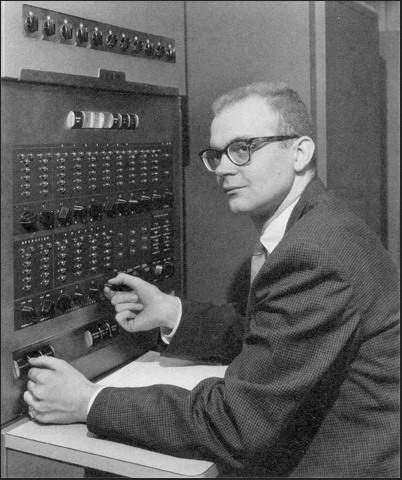
\includegraphics[width=0.9\textwidth]{./media/Don-Knuth-ibm-650-1958.jpg}
    \column{0.6\textwidth}
        \begin{quote}
This series of books is affectionately dedicated to the Type 650 computer once installed at Case Institute of Technology, in remembrance of many pleasant evenings.
        \end{quote}
        \cite{Knuth1973Art}
  \end{columns}
\end{frame}

\section{Art, Creativity and Programming}

\begin{frame}[fragile]
  \frametitle{Art, Creativity and Programming}
  \framesubtitle{subtitle}
  Knuth's sense of art\cite{Knuth1974Computer}

    \begin{quote}
    The process of preparing programs for a digital computer is especially attractive, not only because it can be economically and scientifically rewarding, but also because it can be an \textbf{aesthetic experience much like composing poetry or music}. [emphasis added]
    \end{quote}
    \cite[v]{Knuth1974Computer}
\end{frame}

\begin{frame}
  \frametitle{Neural Plasticity - brains and more}
  \begin{center}
    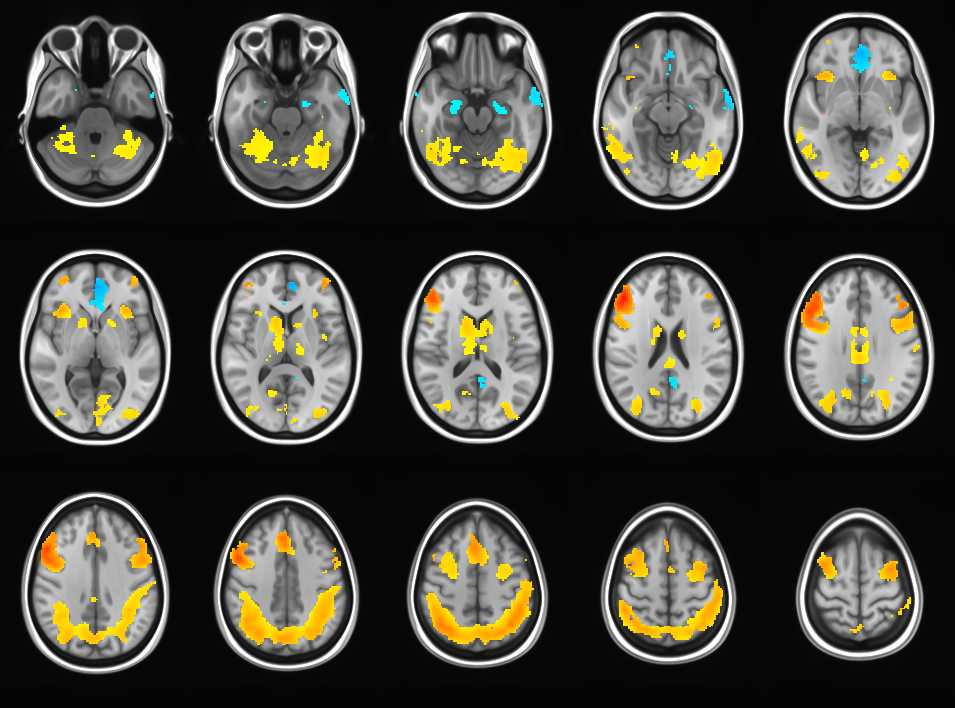
\includegraphics[height=0.75\textheight]{./media/fmri-example.png}
  \end{center}
\end{frame}



\begin{frame}[fragile]{}

  The \themename theme is a Beamer theme with minimal visual noise
  inspired by the \href{https://github.com/hsrmbeamertheme/hsrmbeamertheme}{\textsc{hsrm} Beamer
  Theme} by Benjamin Weiss.

  Enable the theme by loading

  \begin{verbatim}\documentclass{beamer}
    \usetheme{metropolis}\end{verbatim}

  Note, that you have to have Mozilla's \emph{Fira Sans} font and XeTeX
  installed to enjoy this wonderful typography.
\end{frame}

{%
\setbeamertemplate{frame footer}{My custom footer}
\begin{frame}[fragile]{Frame footer}
    \themename defines a custom beamer template to add a text to the footer. It can be set via
    \begin{verbatim}\setbeamertemplate{frame footer}{My custom footer}\end{verbatim}
\end{frame}
}

\begin{frame}{References}
  \cite{Tanaka2013Larger}
\end{frame}

\section{Conclusion}

\begin{frame}{Summary}

  Get the source of this theme and the demo presentation from

  \begin{center}\url{github.com/matze/mtheme}\end{center}

  The theme \emph{itself} is licensed under a
  \href{http://creativecommons.org/licenses/by-sa/4.0/}{Creative Commons
  Attribution-ShareAlike 4.0 International License}.

  \begin{center}\ccbysa\end{center}

\end{frame}

\begin{frame}[standout]
  Questions?
\end{frame}

\appendix

\begin{frame}[fragile]{Backup slides}
  Sometimes, it is useful to add slides at the end of your presentation to
  refer to during audience questions.

  The best way to do this is to include the \verb|appendixnumberbeamer|
  package in your preamble and call \verb|\appendix| before your backup slides.

  \themename will automatically turn off slide numbering and progress bars for
  slides in the appendix.
\end{frame}

\begin{frame}[allowframebreaks]{References}
  \printbibliography

\end{frame}

\end{document}
